\chapter{Теоретичні відомості}

\section{Нахождение абсолютного расстояния методом бинокулярного параллакса}

\subsection{О камерах}
	В нашем случае в качестве ''глаза'' используется камера, поэтому для последующих выкладок нам нужно иметь представление о том, как она устроена и как работает.
	
	Сегодня существует множество разных типов камер, и хоть каждая из них может иметь свои особенности конструкции, базовый принцип работы у них у всех одинаковый.
	
	Основа камеры -- её светочувствительная матрица. В ней свет преобразуются в поток цифровых данных, непосредственно формируя изображение. После неё обычно находится объектив. Он отвечает за проекцию изображения на матрицу, позволяя регулировать фокусное расстояне, значение диафрагмы и другие параметры. 
	
		\includegraphics[scale = 0.75]{camera3}
		
	В рамка этой работы, нам будет достаточно рассмотреть камеру самой простой конструкции. $Pinhole camera$ или же $$!!!Камера обскура!!!$$ -- одна из самых первых "камер". В такой камере отсутствует линза, вместо неё выступает маленькое отверстие в передней части камеры.
	
		\includegraphics[scale = 0.75]{camera_obs+++++++++++++++++++++++++++++++++++++++-----------------------------------------------------------uro}

	В силу оптических особенностей, конечное изображение в такой камере будет перевернутым. Поэтому для ещё большего упрощения мысленно перенесём матрицу камеры направо, на рассояние $f$. Такое действие никак не повлияет на итоговый результат, но сильно упростит дальнейшие выкладки.

	Покажем теперь, как с помощью двух таких камер можно найти абсолютное расстояние до объекта. 
Пусть пока камеры будут рассположены паралельно и сонаправлены друг другу (что делать в случае когда камеры рассположены иначе будет указано дальше).
	Итак, у нас есть такая конструкция:
	
		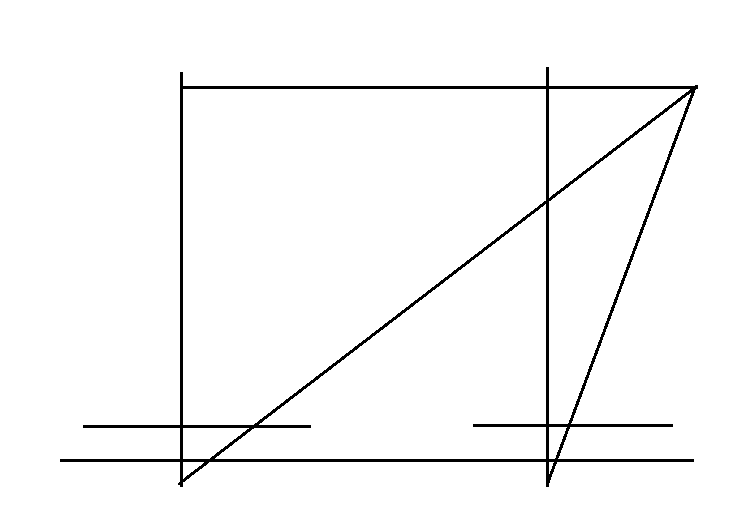
\includegraphics[scale = 0.75]{geometry5}
	
	Где $f$ -- фокусное расстояние камеры, $\Delta$ -- расстояние между камерами, $z$ -- искомая глубина изображения, $x_1, x_2$ -- координата объекта на левом и на правом снимке, $R, L$ -- оптические центры правой и левой камеры, $S$ -- объект.\\
	
	Тогда из подобия треугольников следует:\\
	$$\begin{cases} \frac{f}{x_1} = \frac{z}{\Delta + x} \\ \frac{f}{x_2} = \frac{z}{x} \end{cases}$$
	
	Выразив $\Delta$ из первого уравнения, и $x$ из второго получим:\\
	$$\begin{cases} \Delta = \frac{z x_1}{f} - x \\ x = \frac{zx_2}{f} \end{cases}$$
	
	Подставим $x$ в первое уравнение и выразим из получившегося $z$\\
	$$ z = \frac{\Delta f}{(x_1 - x_2)}$$
	
	Так как $\Delta$ и $f$ не зависят от расположения объекта, а являются характеристиками самой камеры, то расстояние до объекта зависит только от разницы $x_1 - x_2$, то есть только от смещения объекта между двумя снимками. Следовательно для нахождения карты глубин нам нужно найти "сдвиг" для каждого пикселя.\\
	
\subsection{!!Ректификация!!}	
	Но для того чтобы вычислить $x_1 - x_2$ нужно сначала найти эту пару соответствующих пикселей, а это сложная задача. Для каждого пискселя левого изображения, нам нужно найти соответствующий среди пикселей правого изображения. Нужно ли нам перебирать все пиксели правого изображения, или всё таки можно ограничиться каким-то подмножеством пикселей?\\
	
	Пусть у нас есть изображение какого-то объекта на фоне стены.
	$$Рисунок 6$$
	
	Всё что мы можем сказать о его рассположении относительно камеры, это что он находится где-то на луче $L$.
	
	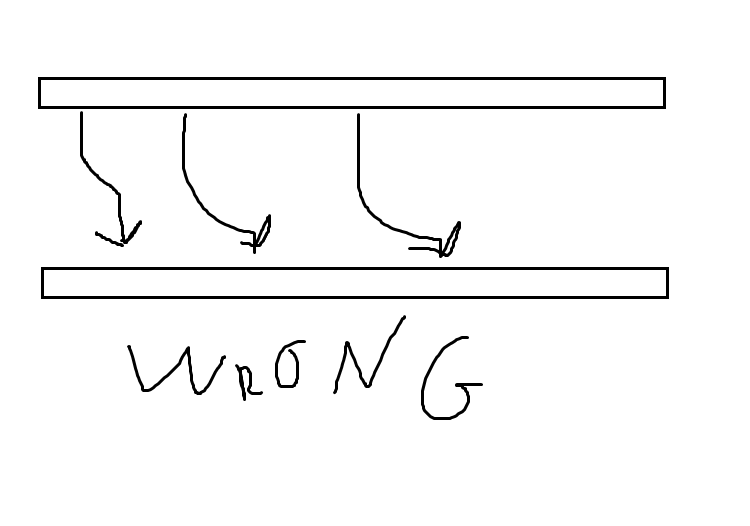
\includegraphics[scale = 0.75]{epipolar}
	
	Добавим теперь вторую камеру, на каком-то расстоянии $\Delta$ от первой камеры. Если мы теперь проведем лучи из оптического центра правой камеры так, чтобы они пересекали луч $L$ - мы получим, так называемые, "эпиполярные линии". И теперь мы можем сократить множество для поиска соответствующих пар со всего изображения до эпиполярных линий на нём. Это существенно облегчает нам задачу.
	
	
\section{Стереозрение при полных данных}
	тест тест тест тест тест тест тест тест тест тест тест тест тест тест тест тест тест тест тест тест тест тест тест тест тест тест тест тест тест тест тест тест тест тест тест тест тест тест тест тест тест тест тест тест тест тест тест тест тест тест тест тест тест тест тест тест тест тест тест тест 
	
	\subsection{Одномерный случай}
	Для простоты рассмотрим алгоритм решения задачи стереозрения в случае когда наши изображения представляют собой строки пикселей. 
	Нам нужно каждому пикселю из левой строки поставить в соответствие пиксель из правой:
	
	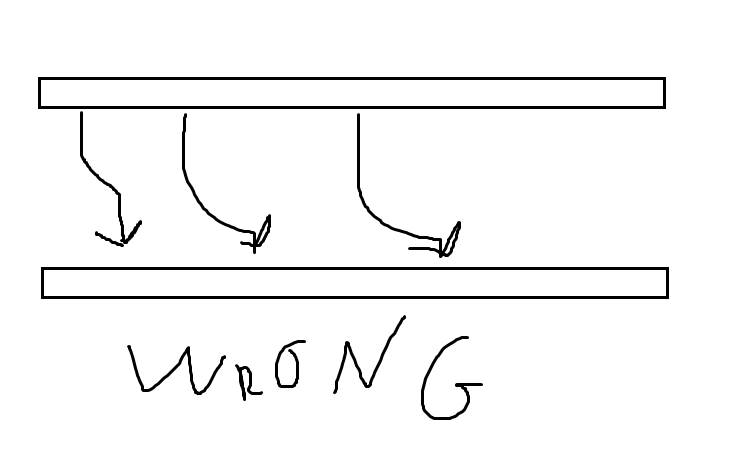
\includegraphics[scale = 0.75]{8}

	Однако не любая пара пикселей может находиться в соответсвии! Пикселю левого изображения с номером $i$ могут соответсвовать только $i-k$ -е  пиксели правого изображения ($k = (0,i-1)$). Вы можете убедиться в этом держа перед собой карандаш и поочередно закрывая то правый, то левый глаз. В правом глазу карандаш будет находиться левее чем в левом.
	$$Рисунок 9$$
	
	
	Но всё же, как нам искать соответствующие пиксели? Какими характеристиками обладают соответствующие пиксели? Логично было бы предположить, что у них одинаковый цвет. Но этого не достаточно. Тогда можно ещё посмотреть какие свойства есть у соседних соответствующих пикселей. Допустим для пикселя $x_{i}$ уже найден соответствующий ему пиксель, то есть нам уже известне сдвиг для $(i)$-го пикселя. Можем ли мы что-то сказать о сдвиге для $(i+1)$-го пикселя? Так как всё же большинство объектов в реальной жизни - гладкие, то велика вероятность, что сдвиг для $(i+1)$-го пикселя не будет сильно отличаться от сдвига $(i)$-го пикселя. Иными словами в последовательности сдвигов должно быть мало скачков.\\
	
	Итак, у нас есть два признака похожести пикселей: схожесть цветов и схожесть соседних сдвигов. Введём качественные оценки этих двух характеристик. Схожесть цветов определим как расстояние между ними, в их цветовом пространстве (!опасный момент!). Схожесть же соседних сдвигов определим просто как модуль разности значений этих сдвигов.\\
	
	Поставим задачу более формально. Пусть множество 
	$\mathcal{L} = \{x_i \; | \; i = \overline{1,\, n}\}$ --- левое изображение-строка, $n$ - ширина изображения, $x_i$ - цвет пикселя (если у нас черно-белые 8-битные изображения, то $x_i \in [ \, 0, \; 255 \,]$, если же цветные, то $x_i \in {[ \, 0, \; 255 \,]}^3$). Введём функцию $\mathcal{L}(i)$ --- цвет $i$-го пискеля на левом изображении. Аналогично, $\mathcal{R}$ --- правое изображение-строка, а $\mathcal{R}(i)$ --- цвет $i$-го пискеля на правом изображение.
	
	Для каждого пикселя $i$ левого изображения нам нужно найти соответствующий ему пиксель на правом изображении, то есть найти такой сдвиг $d_i$, что:
	\begin{enumerate}
	
	\item Мимимизирует \textbf{Унарный штраф} $H(i, d) = | \, \mathcal{L}(i)- \mathcal{R}(i - d) \, |$\\
	(!норма, а не модуль!)
	
	\item Мимимизирует \textbf{Бинарный штраф} $g(d, d') = \alpha \, | \; d - d' \; |$ \\
	(где  --- $\alpha$ коэффициент сглаживания, и подбирается экспериментально)
	
	\end{enumerate}
	
			
	
	Можем построить штрафную функцию 
	$\omega (\overline{d}) = \sum\limits_{i=1}^n H(i, d_i) + \sum\limits_{i=1}^{n-1} g(d_i, d_{i+1})$
	
	Тогда, такая последовательность $\overline{d}$ которая минимизирует штрафную функцию $\omega (\overline{d})$ и будет нашим решением. Таким образом имеем задачу оптимизации.
	
	Для нахождения эффективного решения, и большего понимания задачи,  представим её в несколько ином виде, а именно в виде ориентированного графа. 
	
	Множество вершин $V = \{ \; \sigma(i, d) \, | \, i = \overline{(1,\, n)}, \, d = \overline{(0, \, maxD )} \; \} \bigcup \{\,S, E\,\}$.\\
	Вес вершины $\sigma(i, d) = H(i, d) \;, \; i = \overline{(1,\, n)}, \, d = \overline{(0, \, maxD )}$\\
	Веса ребёр: 
	\begin{enumerate}
	\item Из $S$ в $\sigma(1, d)$ вес ребра = $0$, $d = \overline{(0,\, maxD)}$
	\item Из $\sigma(n, d)$ в $E$ вес ребра = $0$, $d = \overline{(0,\, maxD)}$
	\item Из $\sigma(i, d)$ в $\sigma(i+1, d')$ вес ребра = $q(d, d')$, $d, d' = \overline{(0,\, maxD)}$
	\end{enumerate}	
	
	Получается такой граф:
	$$Рисунок 10$$

 	
 	Тогда, длина пути из вершины $S$ в вершину $E$ через вершины $\sigma(i, d)$ где $i = \overline{(1,\, n)}$, а $d \in \overline{d}$ будет равна:
 	$$\sum\limits_{i=1}^n H(i, d_i) + \sum\limits_{i=1}^{n-1} g(d_i, d_{i+1})$$
 	
	Что в точности повторяет нашу штрафню функцию, причём последовательность $\overline{d}$ минимизирующая эту штрафню функцию, будет отвечать последовательности вершин, которые составляют самый короткий путь из вершины $S$ в вершину $E$.
	
	Таким образом наша задача сводится к поиску кратчайшего пути на графе.\\
	
	Решать эту задачу традиционными алгоритмами типа Белмана-Форда или Дейкстры - не самая лучшая идея. Алгоритм Белма-Форда имеет сложность $|V| * |E|$, причём $|E|$ у нас равна $D^2 n$, где $D$ - максимальный диспаритет, $n$ - ширина изображения.
	
	Куда эффективнее решать эту задачу при помощи ДИНАМИЧЕСКОГО ПРОГРАМИРОВАНИЯ. \\
	
	Обозначим длину кратчайшего пути из вершины S в вершину $\sigma(i, d)$ как $f_i(d)$. 
	Тогда для любого $d \in D$:\\
	
		$f_1(d) = H(1, d)$
		
		$f_2(d) = \min(H(1,d') + g(d', d)) = \min(f_1(d') + g(d', d)) + H(2,d)$
		
	 	...
	 	
	 	$f_n(d) = \min(f_{n-1}(d') + g(d', d)) + H(n,d)$\\

	А саму последовательность $\overline{d}$ находим так:\\
	
		$d_m = arg\min_{d'} (f_m(d'))$
		
		$d_i = arg\min_{d'} (f_i(d') + H(i,d'))$
	
\subsection{Двумерный случай}	
	Двумерный случай Двумерный случай Двумерный случай Двумерный случай Двумерный случай Двумерный случай Двумерный случай Двумерный случай Двумерный случай Двумерный случай Двумерный случай Двумерный случай Двумерный случай Двумерный случай Двумерный случай Двумерный случай Двумерный случай Двумерный случай Двумерный случай Двумерный случай Двумерный случай Двумерный случай Двумерный случай Двумерный случай Двумерный случай Двумерный случай Двумерный случай Двумерный случай Двумерный случай Двумерный случай Двумерный случай Двумерный случай Двумерный случай Двумерный случай Двумерный случай Двумерный случай Двумерный случай Двумерный случай Двумерный случай Двумерный случай Двумерный случай Двумерный случай Двумерный случай Двумерный случай Двумерный случай Двумерный случай Двумерный случай Двумерный случай Двумерный случай Двумерный случай Двумерный случай Двумерный случай Двумерный случай 
	
	
	
\section{Стерезрение при неполных данных}
	Принятие решения при неполных данных 
	


\section{Предвычисления на неполных данных}

	\subsection{Одно изображение известно полностью}
	
	\subsection{Оба изображения известны неполностью}
